% Author       : James Mnatzaganian
%%%%%%%%%%%%%%%%%%%%%%%%%%%%%%%%%%%%%%%%%%%%%%%%%%%%%%%%%%%%%%%%%%%%%%%%%%%%%%%
%TODO:
% * Clean up Abstract for flow
% * Simulation and Modeling Subsection?
% * TM marker on Suricata?
% * Focus on the intricate dependencies that GAN can learn as reason to research (Intro)
% * Helps us understand the limitations of GAN and why it's a good choice for complex alert data (Intro? Methodology?)
% * Illustrate the challenge, address the ways to go about it, show that it works (Methodology)
% *
% *
% *
% *
% *
% *
% *
% *
% *
% *
% *
% *
% *
% *
% *
%%%%%%%%%%%%%%%%%%%%%%%%%%%%%%%%%%%%%%%%%%%%%%%%%%%%%%%%%%%%%%%%%%%%%%%%%%%%%%%
% \begin{document type}
%%%%%%%%%%%%%%%%%%%%%%%%%%%%%%%%%%%%%%%%%%%%%%%%%%%%%%%%%%%%%%%%%%%%%%%%%%%%%%%
% Document Type
%%%%%%%%%%%%%%%%%%%%%%%%%%%%%%%%%%%%%%%%%%%%%%%%%%%%%%%%%%%%%%%%%%%%%%%%%%%%%%%

% Define the document type
\documentclass[cmpe]{ritthesis}
% \end{document type}\end{}

\def\Reals{\mathbf{R}}
\def\Ints{\mathbf{Z}}
\def\Nats{\mathbf{N}}
\def\E{\mathbb{E}}
\def\Q{\mathbb{Q}}
\def\P{\mathbb{P}}
\def\A{{\cal A}}

% \begin{packages}
%%%%%%%%%%%%%%%%%%%%%%%%%%%%%%%%%%%%%%%%%%%%%%%%%%%%%%%%%%%%%%%%%%%%%%%%%%%%%%%
% Packages
%%%%%%%%%%%%%%%%%%%%%%%%%%%%%%%%%%%%%%%%%%%%%%%%%%%%%%%%%%%%%%%%%%%%%%%%%%%%%%%

% Used for creating clicking references
\usepackage[hidelinks]{hyperref}

% Used for displaying images
\usepackage{graphicx}

% Support for typesetting math
\usepackage{mathtools}

% Support for number sets
\usepackage{amsfonts}

% Support for logic notation
\usepackage{amssymb}

% Support for typesetting subcaptions
\usepackage{subcaption}

% Typset indexes - Needed for sorting the glossary
%  - xindy: Sorting / indexing of items
\usepackage[xindy]{imakeidx}

% Support for glossaries
%  - nopostdot: Omit dot at the end of each description
%  - nonumberlist: Supress number of items
%  - acronym: Support for acronyms
%  - toc: Add glossary to table of contents
%  - xindy: Sorting / indexing of items
\usepackage[nopostdot,nonumberlist,acronym,toc,xindy]{glossaries}

% Support for displaying pseudo-code
\usepackage{algorithm}

% Support for displaying pseudo-code
%  - noend: Don't display end ...
\usepackage[noend]{algpseudocode}

% Support for pretty inline fractions
\usepackage{nicefrac}

\usepackage{times}
\usepackage{lscape}
\usepackage{verbatim}
\usepackage{enumerate}

% \end{packages}

% \begin{macros}
%%%%%%%%%%%%%%%%%%%%%%%%%%%%%%%%%%%%%%%%%%%%%%%%%%%%%%%%%%%%%%%%%%%%%%%%%%%%%%%
% Macros
%%%%%%%%%%%%%%%%%%%%%%%%%%%%%%%%%%%%%%%%%%%%%%%%%%%%%%%%%%%%%%%%%%%%%%%%%%%%%%%

% Default header for a table
\newcommand{\tableheader}[1]{\multicolumn{1}{|c|}{\textbf{#1}}}

% Section referencing
\newcommand{\sref}[1]{Section~\ref{#1}}

% Figure referencing
\newcommand{\fig}[1]{Figure~\ref{#1}}

% Equation referencing
\newcommand{\eq}[1]{(\ref{#1})}

% Algorithm referencing
\newcommand{\alg}[1]{Algorithm~\ref{#1}}

% Glossary referencing
\newcommand{\glsref}[1]{\\ \textit{Glossary:} \gls{#1}}

% Change comment style to use #
\algrenewcommand{\algorithmiccomment}[1]{\# #1}

% Make *proper* vector arrows - Credit to harpoon pacakge for initial idea
\newlength{\argwd}
\newlength{\arght}
\newcommand{\overharp}[3]{%
	\settowidth{\argwd}{#2}%
	\settoheight{\arght}{#2}%
	\addtolength{\argwd}{.1\argwd}%
	\raisebox{\arght}{%
		\makebox[.04\argwd][l]{%
			\resizebox{\argwd}{#3\arght}{$#1$}%
		}%
	}%
	#2%
}
\newcommand{\overrightharp}[2]{\overharp{\rightharpoonup}{#1}{#2}}
\newcommand{\vect}[2][.5]{\text{\overrightharp{\ensuremath{\boldsymbol{#2}}}{#1}}}
\newcommand{\vectmd}[2][.5]{\text{\overrightharp{\ensuremath{#2}}{#1}}}

% Make *proper* text over sim - Credit: http://tex.stackexchange.com/a/43338/66603
\newsavebox{\mybox}\newsavebox{\mysim}
\newcommand{\distas}[1]{%
  \savebox{\mybox}{\hbox{$\scriptstyle#1$}}%
  \savebox{\mysim}{\hbox{$\sim$}}%
  \mathbin{\overset{#1}{\resizebox{\wd\mybox}{\ht\mysim}{$\sim$}}}%
}

%%  Collection of useful abbreviations.
\newcommand{\etc} {\emph{etc.\/}}
\newcommand{\etal}{\emph{et~al.\/}}
\newcommand{\eg}  {\emph{e.g.\/}}
\newcommand{\ie}  {\emph{i.e.\/}}
% \end{macros}

% \begin{document configuration}
%%%%%%%%%%%%%%%%%%%%%%%%%%%%%%%%%%%%%%%%%%%%%%%%%%%%%%%%%%%%%%%%%%%%%%%%%%%%%%%
% Document Configuration
%%%%%%%%%%%%%%%%%%%%%%%%%%%%%%%%%%%%%%%%%%%%%%%%%%%%%%%%%%%%%%%%%%%%%%%%%%%%%%%

% Add DRAFT to the document
%\usepackage{draftwatermark}
%\SetWatermarkText{DRAFT}
%\SetWatermarkScale{9}
%\SetWatermarkColor[gray]{0.90}
%\SetWatermarkAngle{45}

% Set the path for the figures
\graphicspath{{figs/}
	{01_introduction/figs/}
	{02_related_works/figs/}
	{03_methodology/figs/}
	{04_design_implementation/figs/}
	{05_results_and_analysis/figs/}
}

% Author, title, and date
\author{Christopher R. Sweet}
\title{Applying Generative Adversarial Networks to Cyber-Alert Data}
\date{April 2019}

% Advisor details
\advisor{Professor}{Dr. Shanchieh}{Yang}
\committee{Assistant Professor}{Dr. Raymond}{Ptucha}{}
\committee{Associate Professor}{Dr. Sonia}{Lopez-Alarcon}{}
% \end{document configuration}\end{}

% \begin{glossary}
%%%%%%%%%%%%%%%%%%%%%%%%%%%%%%%%%%%%%%%%%%%%%%%%%%%%%%%%%%%%%%%%%%%%%%%%%%%%%%%
% Glossary Setup
%%%%%%%%%%%%%%%%%%%%%%%%%%%%%%%%%%%%%%%%%%%%%%%%%%%%%%%%%%%%%%%%%%%%%%%%%%%%%%%

% Load the glossary
\loadglsentries{glossary}

% Load the acronyms
\loadglsentries[type=\acronymtype]{acronym}

% Initialize the glossary
\makeglossaries
\setglossarystyle{altlist}

% Sort the glossary
\makeindex
% \end{glossary}

% \begin{document}
%%%%%%%%%%%%%%%%%%%%%%%%%%%%%%%%%%%%%%%%%%%%%%%%%%%%%%%%%%%%%%%%%%%%%%%%%%%%%%%
% Document Start
%%%%%%%%%%%%%%%%%%%%%%%%%%%%%%%%%%%%%%%%%%%%%%%%%%%%%%%%%%%%%%%%%%%%%%%%%%%%%%%

\begin{document}
	
	% Pre chapter stuff
	\frontmatter
% \begin{acknowledgments}
%%%%%%%%%%%%%%%%%%%%%%%%%%%%%%%%%%%%%%%%%%%%%%%%%%%%%%%%%%%%%%%%%%%%%%%%%%%%%%%
% Acknowledgments
%%%%%%%%%%%%%%%%%%%%%%%%%%%%%%%%%%%%%%%%%%%%%%%%%%%%%%%%%%%%%%%%%%%%%%%%%%%%%%%

\begin{acknowledgments}
	\vfill
	\begin{center}
		\indent Most importantly, thank you to Dr. S. Jay Yang for providing me with the opportunity to assist in research throughout my undergraduate study. Your continued feedback and encouragement to challenge myself over the years has helped me to grow into a strong engineer and critical thinker. You have had a profound impact on me, and I can never thank you enough for that. Next, I would like to thank Dr. Raymond Ptucha, Dr. Sonia Lopez-Alarcon, and the rest of the RIT Computer Engineering faculty for their willingness to educate the next generation of Computer Engineers. Finally, I would like to thank (the soon to be Dr.) Stephen Moskal who provided me my first opportunity to research with him and Dr. Yang when I was in my second year of undergrad. The advice, feedback, and good times over the last few years have been invaluable. 
	\end{center}
	\vfill
\end{acknowledgments}
% \end{acknowledgments}

% \begin{dedication}
%%%%%%%%%%%%%%%%%%%%%%%%%%%%%%%%%%%%%%%%%%%%%%%%%%%%%%%%%%%%%%%%%%%%%%%%%%%%%%%
% Dedication
%%%%%%%%%%%%%%%%%%%%%%%%%%%%%%%%%%%%%%%%%%%%%%%%%%%%%%%%%%%%%%%%%%%%%%%%%%%%%%%

\begin{dedication}
	\vfill
	\begin{center}
		To my mother and father, Debbie and Jack Sweet, who taught me the value of a strong work ethic. And to my brother, John, who always set an extremely high bar for me to try and beat. Without your continued support, guidance, and devotion, I never would have been able to achieve all that I have. 
	\end{center}
	\vfill
\end{dedication}
% \end{dedication}

%\begin{abstract}
%%%%%%%%%%%%%%%%%%%%%%%%%%%%%%%%%%%%%%%%%%%%%%%%%%%%%%%%%%%%%%%%%%%%%%%%%%%%%%%
% Abstract
%%%%%%%%%%%%%%%%%%%%%%%%%%%%%%%%%%%%%%%%%%%%%%%%%%%%%%%%%%%%%%%%%%%%%%%%%%%%%%%

% Abstract
\begin{abstract}
	% Focus on the challenge of creating cyber alert data in abstract
	% Second paragraph is more about methods and uniqueness
	
	Cyber attacks perpetrated against enterprise computer networks continue to grow in number, severity, and complexity as our reliance on such networks grows. Despite this, proactive cyber security remains an open challenge as cyber alert data is often not available for study. Furthermore, the data that is available is stochastically distributed, imbalanced, lacks homogeneity, and relies on complex interactions with latents aspects of the network structure. Currently, there is no commonly accepted way to model and generate synthetic alert data for further study; there are also no metrics to quantify the fidelity of synthetically generated alerts or identify critical attributes within the data.
	
	This work proposes solutions to both the modeling of cyber alerts and how to score the fidelity of such models. Generative Adversarial Networks are employed to generate cyber alert data taken from two collegiate penetration testing competitions. A list of criteria defining desirable attributes for cyber alert data metrics is provided. Several statistical and information-theoretic metrics, such as histogram intersection and conditional entropy, meet these criteria and are used for analysis. Using these metrics, critical relationships of synthetically generated alerts may be identified and compared to data from the ground truth distribution. Finally, through these metrics we show that adding a mutual information constraint to the model's generation increases the quality of outputs and successfully captures alerts that occur with low probability.
	
\end{abstract}

%%%%%%%%%%%%%%%%%%%%%%%%%%%%%%%%%%%%%%%%%%%%%%%%%%%%%%%%%%%%%%%%%%%%%%%%%%%%%%%
% Introductory Lists and Tables
%%%%%%%%%%%%%%%%%%%%%%%%%%%%%%%%%%%%%%%%%%%%%%%%%%%%%%%%%%%%%%%%%%%%%%%%%%%%%%%

% Add TOC, list of figures, list of tables in that order
\makealllists

% Add the acronyms
\glsaddall
\printglossary[type=\acronymtype]


% Reset all acronyms
\glsresetall

% Start using Arabic numbers
\mainmatter
% \end{introductory lists and tabels}
	
	% Actual chapters
	\chapter{Introduction}

\section{Network Intrusion Detection Systems}
A variety of packet capture tools exist to enable individuals and corporations alike to monitor traffic on their networks. Several tools take this logging a step further and allow for real time network intrusion detection. Network intrusion detection systems (NIDS) are a rule based system which allows for automated flagging of potentially malignant packet traffic through the aggregation of temporally contiguous packets;  these alerts typically consist of the believed attack signature, a category that the attack falls under, target machine, timestamp, and more. These systems are employed to flag potentially malicious traffic, note long term patterns in traffic, and provide system administration with a trail of alerts to analyze after a cyber-attack has taken place. 

Though these tools provide network operators with a wealth of data to analyze they suffer from a fundamental issue. The data only exists after a cyber attack has already taken place, and therefore only allows for reactionary defense techniques. This has lead researchers to see if they can use this data, as well as simulations and extrapolation, to further understand network vulnerabilities in the pursuit of proactive cyber security. 

\section{Challenges of Cyber Alert Data}
Cyber Alert data suffers from two primary challenges; There is a lack of malicious traffic data and the data that does exist is imbalanced, non-homogeneous, and unlabeled. 

Access to malicious NIDS alert data has been a long standing problem for researchers in the domain of Cyber Security. As an alternative probablistic models, such as attack graphs \cite{Qin2004, Wang2006, Noel2009}, have been proposed and updated to try and create realistic attack data for varying network architectures in an automated fashion. These models provide insight into potential attack paths within a network, the probability a given path will be used, and what vulnerabilities within the network allow for these paths to exist. Other works have defined methods to model these attack graphs as Markov Chains \cite{Li2017}, while others have employed statistical graph models \cite{Du2014} and Variable Length Markov Models \cite{Fava2008} in attempts to better understand potential vulnerabilities. Despite the effectiveness of these models however they lack any means to consider historical attack data or consider real network alerts. 

Of the datasets which do exist, common issues include small data set size, high imbalance between malignant and benign alerts, redundant samples, and intricate interactions leading to misleading labels. One example of this is the KDD Cup '99 \cite{kdd-cup} dataset. This dataset was prepared by Stolfo \etal \cite{Stolfo} based off data captured in DARPA'98 IDS evaluation program \cite{Lippmann}. It consists of samples from 7 weeks of network traffic collected via TCPdump that was labeled with one of 5 labels {normal, denial of service, user to root attack, remote to local attack, or probing attack}. Recently, it been used for multiple studies involving cyber attack classification and prediction through the use of recurrent neural networks (RNNs) \cite{Kim, Staudemeyer}. However this dataset contains several pathological issues such as synthetic background traffic, underlying issues with TCPdump under intense load, and a lack of precise definitions for what constitutes an attack, as highlighted by Tavallaee \etal \cite{Tavallaee} and McHugh \cite{McHugh}.

Other publicly available datasets struggle with a low signal to noise ratio. Two examples of this are the Multi Source Cyber Event Dataset published by Los Alamos National Laboratory \cite{akent-2015-enterprise-data} and the DeepSecurity Dataset released by Faber and Malloy \cite{Faber2018}. The Multi Source Cyber Event Dataset contains 4.8 KB of textual information pertaining to malicious events. The magnitude of these events pales in comparison to the overall scale of the dataset, which is encompassed in 12.2 GB of textual data. DeepSecurity faces a similar issue with a low percentage of their 600,000 network events being representative of malicious network traffic. The authors note that the availability of quality labeled data and a low signal to noise ratio for malicious activity are both outstanding issues with their studies \cite{Faber2018}. 

Though the distribution of malicious events in these datasets may be representative of real world cyber alert data it creates many challenges for network defense. These challenges include the potential obfuscation of attack behavior, difficulty isolating malicious alerts interspersed throughout a stream of non-malicious alerts, and no ground truth labels. With no commonly accepted means to artificially generate additional malicious alert data, these challenges persist in the field of Cyber Security. 

\section{Generative Adversarial Networks}

A Generative Adversarial Network (GAN) is a class of neural network where two neural networks are pitted against each other. One network, the generator, attempts to create samples which seem to belong to a ground truth dataset. The other network, the discriminator, takes inputs from the ground truth dataset as well as the generator and flags samples as either real or fake. This structure minimizes the generator loss each time the generator successfully creates a sample that tricks the discriminator into marking the sample as real. Conversely, the discriminator loss is minimized when all samples from the ground truth set are marked as real and all samples created by the generator are marked as fake.

GANs have achieved state of the art results in generating data with respect to images \cite {Karras2018, Zhu2017, Ledig2016}, text \cite{Su2018}, and sound \cite{Dong2018, Gao2018}.  Additionally, they have also been shown to perform well at more complex tasks such as scene to scene translation in images \cite{Zhu2017, Choi2017} and stylized image generation \cite{Karras2018}. These architectures allow GANs to serve as a powerful tool to artificially expand datasets. Additionally, high fidelity data generation requires the generator to learn key dependencies between features within each generated sample. A means to reveal and analyze these dependencies would be a powerful tool for analyzing critical features within the dataset.

Despite these successes, GANs do have several shortcomings. They are noted for requiring large numbers of samples per class and are typically trained across very large datasets for many epochs. The loss functions do not represent the quality of the data, as both the generator and discriminator are continually learning; as one network becomes better it's loss may drop, only to rise back up in a few batches when the other network learns something new as well. This lack of convergence makes training and hyperparameter tuning even more important than in traditional Deep Learning models. Allowing one model to overpower the other starves the system from having any useful gradient feedback. Finally, output mode dropping may occur, as the generator may not receive sufficient gradient feedback to encourage full exploration of the dataset.

\section{Problem Statement}

In order to address the lack of malicious NIDS alert data for cyber attack studies, we explore the usage of GANs as a means to recreate and expand existing alert data. The application of GANs is challenged by potential for output mode collapse and failure of the network to learn realistic output distributions for each feature. Generalized preprocessing techniques are defined to prepare NIDS alert data for usage with GANs while also making model inputs and outputs more intuitive to analysis. 

Since there is no commonly accepted metric to score the fidelity of synthetically generated alerts, several desirable attributes for alert fidelity scoring are defined. Subsequently, histogram intersection and Jensen Shannon divergence are proposed as metrics which meet these criteria and are used to evaluate synthetically generated alerts from a GAN. Advantages and disadvantages of each metric are reviewed. 

Furthermore, conditional entropy and joint entropy are suggested as means to measure the efficacy of the GAN on learning the intricate feature interactions within an alert. Conditional probability tables are also employed to further understand the degree to which GANs learn feature dependencies. These methods provide insight into the critical features of alert data even when applied outside the context of analyzing synthetically generated alerts. Additionally, they provide detailed contextual information by allowing researchers to directly analyze feature-value relationships in alert data. 

Finally, mutual information maximization is proposed as a means to regularize the generators output. This addition encourages further exploration of the ground truth dataset and reduces output mode collapse.  



	
\chapter{Related Work}

With the recent resurgence of Machine Learning research and incredible effectiveness of Deep Learning models, researchers across a variety of domains have begun to apply these methods to outstanding challenges in their fields. Cyber-Security is included in these newfound avenues of research, as Deep Neural Networks have been used for cyber event classification, forecasting, malicious traffic modification, and data generation. This section shall be organized as follows: First, a survey of existing applications of Machine Learning to Cyber Security problems will be reviewed to illustrate the need for rich alert datasets. Then advances in generative models from other fields will be examined to better understand how state of the art generative models achieve such impressive results. And finally, the current use case of generative models for cyber security will be compared to the methods proposed by this work. 

\section{Cyber Security and Machine Learning}

The predominant application of Machine Learning to Cyber Security has been focused on the challenge of anomaly detection, attack classification, and event prediction. For all of these tasks intricate relationships must be considered between the various features of alerts, as well as entire chains of temporally connected alerts. 

In order to maintain these temporal relationships, Recurrent Neural Networks have been employed. Specifically, Long Short Term Memory (LSTM) units allow for the network to learn how to weight the importance of prior events and when to forgot previous feature values entirely. These models have been applied to Cyber Physical Systems by Filonov \etal  to identify anomalous behavior. Their results show that LSTMs are able to outperform traditional methods of anomaly detection such as PCA, FDA, DFDA, CVA and SVM \cite{Filonov2016, Filonov2017}.

Other works make use of the aforementioned KDD Cup'99 dataset for cyber event classification. Both the works of Staudemeyer \etal \cite{Staudemeyer} and Kim \etal \cite{Kim} show that LSTM networks are able to achieve impressive results, with near $100\%$ accuracy when tasked with identifying if a stream of traffic is normal, or falls into one of the four malignant labels. 

Similarly, Tuor \etal \cite{Tuor} use system logs and a twin neural network model to identify if alerts are malignant. The first model extracts information from the past $24$ hours of system logs by embedding a mixture of categorical and event count features into a hidden representation. A series of these hidden representations are then fed into the second model, an LSTM network, which classifies potential cases of malignant behavior. Through the usage of a fixed sliding window the dataset may be continuously updated. This allows for a continuous training approach to be used, keeping models up to date regarding new system log behavior. 

Another example of alert classification is $AI^2$ \cite{Veeramachaneni2016} which integrates expert input into the network traffic used for training an LSTM. The LSTM learns identify anomalous behavior which is then classified by a human analyst. The analyst's feedback is then given to the network and used for future parameter updates so that future events may be flagged with a higher degree of accuracy.

Other works have taken the challenge of prediction and classification a step further and attempted to forecast attributes of future attacks. One example of this is the work of Perry \etal \cite{us} who applied LSTMs to a collegiate penetration testing competition to see if alerts early in the competition could be used to identify which team was perpetrating an attack later on in the event. Further, they also showed that attributes of future attacks could be forecast, such as the alert signature and destination port. 

Similarly Shen \etal \cite{Shen2018} applied LSTMs to a dataset of 3.4 billion security events collected from Symantec's Intrusion Prevention Product deployed on corporate networks which have opted in to it's data sharing program. Their results demonstrate that LSTM can be used to predict target machine, attack severity, and even specific common vulnerability exploits which may be used in the attack with over $80\%$ accuracy. 

All of these systems for attack classification and prediction make use of data collected via NIDS. Despite the promising results of each, several of the authors note that they believe an increased dataset would allow for them to further improve the accuracy of their models \cite{us, Faber2018, Shen2018}. 

\section{Generative Adversarial Networks: Models and Improvements}

First proposed by Goodfellow \etal \cite{Goodfellow2014}, GANs are a game theoretic model for generating increasingly realistic data in a semi supervised manner. Two neural networks, referred to as the generator and the discriminator, are pitted against each other. The generator learns a set of nonlinear transformations ($T$) to apply to noise $\widehat{x}$ sampled from $\P_{\widehat{x}}$. These transformations result in data which imitates that of the ground truth set $x$ sampled from $\P_r$. The discriminator is fed both real,  $x$ sampled from $\P_r$, and generated, $\widetilde{x}$ sampled from $\P_g$, data and assigns a probability $d \in [0,1]$ representing the believed probability that a sample came from the distribution $\P_r$. 

Immediately, GANs proved themselves to be a powerful tool for the generation of new samples in continuous value spaces such as images. Rapid advances came through the application of conditional generation \cite{Mirza2014}, Deep Convolutional Networks \cite{Radford2015}, and Information Theoretic extensions \cite{Chen2016}. 

Simultaneously the training and structure of GANs were updated to improve convergence rates, palliate output mode dropping, and provide meaningful learning curves \cite{Salimans, Arjovsky2017, Gulrajani2017}. Most notably, the Wasserstein GAN (WGAN) proposed by Arjovsky \etal \cite{Arjovsky2017} introduced the usage of the Earthmover Distance as the loss function for both the generator and discriminator. Intuitively, this distance represents how much "mass" must be transported from x to y in order to transform $\P_g$ into $\P_r$. 

WGAN was subsequently improved by Gulrajani \etal \cite{Gulrajani2017} by adding a gradient penalty term (WGAN-GP) to regularize the gradients of D. The gradient penalty creates a 1-Lipschitz constraint on the discriminator during training by sampling noise $\widehat{x}$ from $\P_{\widehat{x}}$ and constraining the gradient of the L2 norm of $D(\widehat{x})$ to 1. Additionally, the discriminator was given real samples and generated samples in a 5:1 ratio per epoch of training; this is done to increase the utility of gradients provided to the generator by discriminator. These modifications to training result in the loss formulation shown in (\ref{eq:WGAN-GP1}), (\ref{eq:WGAN-GP2}), and (\ref{eq:WGAN-GP3}) for the discriminator, the gradient penalty term, and the generator respectively:

\begin{align}
	D_{loss} &=  \E_{\widetilde{x} \thicksim \P_g}[D(\widetilde{x})] - \E_{x \thicksim \P_r}[D(x)] + \label{eq:WGAN-GP1} \\
	& \lambda \E_{\widehat{x} \thicksim \P_{\widehat{x}}}[(||\nabla_{\widehat{x}} D(\widehat{x})||_2 -1)^2] \label{eq:WGAN-GP2}\\
	G_{loss} &=  -\E_{\widetilde{x} \thicksim \P_g}[D(\widetilde{x})] \label{eq:WGAN-GP3}
\end{align}

Note that in the above $\lambda$ is a tunable hyperparameter determining the influence the gradient penalty has on discriminator loss; $\nabla$ is the symbol for the gradient of D($\widehat{x}$); $\E$ is the expectation of the values x sampled from the distribution $\P$.

\begin{equation}
	D_{KL}(P||Q) = \sup\limits_{T:\Omega \rightarrow \Reals} \E_\P[T] - \log(\E_\Q[e^T])
	\label{eq:MINE}
\end{equation}

Separate from the advances of WGAN and WGAN-GP, Mutual Information Neural Estimation (MINE) \cite{Belghazi2018} was introduced as a means to help palliate output mode dropping and improve reconstruction of generative models. MINE uses a neural network optimized using the Donsker-Varadhan representation of the KL-Divergence, given in (\ref{eq:MINE}), to estimate the mutual information $I$ between two distributions. 

Similar to the Earthmover Distance, the KL Divergence is a metric that quantifies the distance between two arbitrary distributions, P and Q. However, the KL divergence makes use of the logarithm to express this distance in units of nats or bits. In the DV representation given in (\ref{eq:MINE}) T is the family of transformations that maps the input features $\Omega$ to $\Reals$. Thus  $\E_\P[T]$ and $\E_\Q[e^T]$ are the distributions whose divergence is being measured by a neural network learning transformations $T$. 

In order to palliate mode dropping by the generator, Belghazi \etal \cite{Belghazi2018} propose to regularize the generator by the negative-entropy of it's output distribution. Since this is often intractable for real world samples the mutual information between the sampled noise and output samples can be used as a proxy.

The Mutual Information estimate is then added to the generator's loss defined in (\ref{eq:WGAN-GP3}), resulting in the formulation given by (\ref{eq:g_loss_new}).

\begin{equation}
G_{loss} =  -\E_{\widetilde{x} \sim \P_g}[D(\widetilde{x})] + D_{KL}(\widehat{x}||\P_g)
\label{eq:g_loss_new}
\end{equation}



\section{Applications of Generative Adversarial Networks to Network Traffic: Adversarial Sample Crafting}

One common application of GANs has been the creation of Adversarial Samples. First noted by Szegedy \etal \cite{Szegedy2013}, Adversarial Samples are generated by taking ground truth samples, applying a small, human-imperceptible, perturbation, resulting in that sample being misclassified by a neural network with a high degree of confidence. Subsequent research found more powerful ways to generate Adversarial Samples through methods such as fast gradient sign \cite{Goodfellow2015}, optimization based methods \cite{Carlini2017, Liu2017, Eykholt2018}, and GANs \cite{Xiao2018, Rigaki2018, Lin2018, Hu2017, Anderson2017}. 

Advarsarial Sample Crafting has been applied to network traffic to modify and obfuscate malicious traffic \cite{Rigaki2018, Lin2018, Hu2017, Anderson2017}. These adversarial samples are created to avoid being flagged by Network Intrusion Detection Systems (NIDS).

Rigaki \etal \cite{Rigaki2018} proposed the use of GANs in generating network traffic which mimics other types of network traffic. In particular, real malware traffic was modified by a GAN using LSTM cells to appear as legitimate network traffic. This allowed the malware to avoid detection from the Stratosphere Behavioral Intrusion Prevention System through the modification of three network traffic parameters; total byte size, duration of network flow, and time delta between current network flow and the last network flow. They showed that through the modification of these parameters detection rate could be dropped down to 0\%. 

Similarly, Lin \etal \cite{Lin2018} apply GANs to obfuscate traffic with the intention of directly deceiving a NIDS. Their model makes use of 9 discrete features and 32 continuous features to modify attack actions to avoid detection. Available attack actions include denial of service and privilege escalation. Their model is shown to drastically increase the evasion rate of malicious network traffic across several different classifiers when benchmarked using the NSL-KDD benchmark provided in \cite{Hu2015}.

\section{Summary}

The current research in applying Machine Learning to Cyber Security is well varied, but missing the application of generative models to new sample creation and analysis. This work applies state of the art GAN models to cyber alert data collected via the Suricata NIDS to fill this gap. The alerts used for training were collected from 10 student teams during an 8 hour long collegiate penetration testing competition (CPTC) as they attacked identical, isolated, instances of the same network topography. Two different years of competition data were tested independently, each representing different network topographies and attacker behaviors; additionally, illustrating the ability of a single network topography to learn and capture many different data distributions. All data was processed to consider traffic a per target IP basis allowing for different models to be used to represent each potential target in the network. 

Unique preprocessing steps for handling cyber alert data, exhaustive model hyperparameter tuning, and methods of identifying generated sample fidelity are also provided. Namely, the usage of Histogram Intersection and Jensen Shannon Divergenc, for m-tuple feature combinations, are shown to be an effective and intuitive means of judging sample generation quality. Additionally, these metrics may be coupled with joint and conditional entropy calculations to show dependencies between features of an alert, allowing for further introspection of attack behavior.

Finally, the application of Mutual Information Estimate Maximization to WGAN-GP is shown to improve sample generation by increasing the number of output modes captured by the generator. This model is referred to as WGAN-GPMI and is shown to improve generated results through a higher intersection of histograms and closer probability distribution approximation by the generator.

	\chapter{Methodology}
\label{sec:meth}

In order to generate and analyze cyber alert data it is important to understand the structure of generic NIDS alerts. The categorical features contained by each alert provide contextual information such as the what, where, and how an attack occurs. By understanding the structure and meaning of each alert feature it is possible to begin selecting which features are worth pursuing synthetic generation of. Furthermore, the selection of these features drives the structure of the generative model used. This section will detail three neural network architectures driven by the features selected from NIDS alerts. 

\section{Alert Structure and Feature Selection}

NIDS alerts are formed through the compilation of packet traffic seen by each machine on the network. These alerts use fixed rulesets and information collected from multiple packets to summarize the believed intent of network traffic. Features such as HTTP Request Information, Alert Category and Signature, Destination IP, Source IP, and more are all captured by alerts. A subset of alert features are shown in Fig. \ref{fig:alert}. 

It is important to note that not all features are populated in every alert and that most features are comprised of discrete categorical values. Additionally, many features are grouped into families of information. One example of this is the HTTP family, which includes Hostname, Method, Redirect, URL, and more.

\begin{figure}
	\centering
	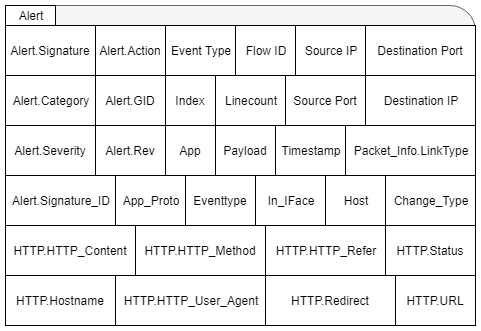
\includegraphics[width=.8\textwidth]{alert_struct}
	\caption{Sample NIDS Alert}
	\label{fig:alert}
\end{figure}

Given the wide variety of alert features available it is important to establish which alerts provide useful contextual information for future network alert modeling. Additionally, some of the features listed are generated through a fixed mapping from other features. For example, Alert Category is determined by a many to one mapping of Alert Signatures. Therefore, by generating Alert Signature it is possible to determine the Alert Category. 

When selecting features of an alert to use for any model it is important to consider the contextual data provided by that features. Features such as Alert Signature, Category, Action, and Eventtype provide the what and how an attack is carried out over the network. Destination IP and Port and Source IP and Port provide where the attack originated from and where it's targeting.  And Timestamp provides not only when an attack occurs but also it's temporal location with respect to other alerts.


\section{GAN Models}
\label{sec:model_arch}
Two GAN implementations were created to generate artificial cyber alert data; a standard Wasserstein GAN with Gradient Penalty and an extension of this model which used a neural estimate of mutual information to regularize the generator output. The mutual information estimate model architecture is also reviewed in detail.

\subsection{Wasserstein GAN with Gradient Penalty}
\label{sec:gan}
The Wasserstein GAN with Gradient Penalty makes no architectural changes to model structure compared to standard GANs. Rather, the loss function is modified to use the Earthmover Distance. This modification has been shown to create empirically better results and allows for flexibility in model selection adapted to the challenge at hand.

Since the goal of this work was to create individual NIDS alerts without temporal correlation a feed-forward network architecture was selected for both the generator and discriminator. Four alert features were selected for alert generation: Alert Signature, Destination Port, Timestamp, and Source IP. Despite this, the models employed could easily be scaled to consider n-many features. 

The generator consisted of 2 layers. The first layer sampled from noise space $\mathbb{Z}$ to a hidden representation. The next layer was directly responsible for each feature's output value. Since each of the four selected features was categorical, one hot encoded representations were used to represent each unique value. This layer consisted of four individual mappings from the hidden representation to an output layer with cardinality equal to the number of unique values per feature. Finally, a concatenation was used to take the prior 4 outputs and create a full 1-hot encoded alert. 

The discriminator also consisted of 2 layers. The first layer took 1-hot encoded alerts as input and mapped them to a hidden representation. The next layer mapped this hidden representation to a scalar value representing the probability that the alert was from the ground truth dataset. A graphical model of this architecture is included in Fig. \ref{fig:model_simple}. Inputs to the network are highlighted in yellow. Learnable weight layers are in blue. The concatenation in orange is a non-backpropable layer used only to prepare generator output for input to the discriminator. And the red boxes and lines represent the model loss functions and back-propagation.

\begin{figure}[!htbp]
	\centering%
	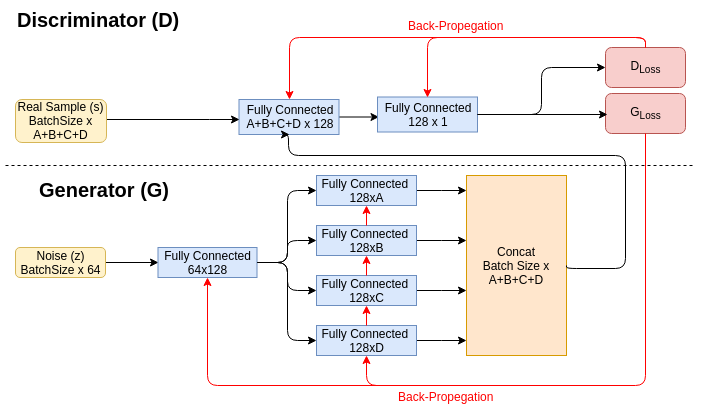
\includegraphics[width=\textwidth]{model_simple}
	\caption{WGAN-GP Model}
	\label{fig:model_simple}
\end{figure}

Table \ref{tab:model_simple_a} and Table \ref{tab:model_simple_b}, shows the dimensions of the weight matrices and activation functions for each layer of the network.

\begin{table}[!htbp]
	\centering
	\caption{Generator Network Architecture: Note that a-d are variable depending on the number of unique outputs}
	\label{tab:model_simple_a}
	\begin{tabular}{l|c|c}
		\hline
		\multicolumn{3}{c}{\textbf{Generator}} \\ 
		\hline
		\multicolumn{1}{c|}{Layer} & \multicolumn{1}{c|}{Matrix Dimensions} & \multicolumn{1}{c}{Activation Function} \\ \hline
		Input & 64 x 128 & {$x^+$} \\
		Output - Feature 0 & 128 x A & NA \\
		Output - Feature 1 & 128 x B & NA \\
		Output - Feature 2 & 128 x C & NA \\
		Output  - Feature 3 & 128 x D & NA \\
		Concatenation & A+B+C+D & NA \\
		\hline
	\end{tabular}
\end{table}

\begin{table}[!htbp]
	\centering
	\caption{Discriminator Network Architecture: Note that a-d are variable depending on the number of unique outputs}
	\label{tab:model_simple_b}
	\begin{tabular}{l|c|c}
		\hline
		\multicolumn{3}{c}{\textbf{Discriminator}} \\ 
		\hline
		\multicolumn{1}{c|}{Layer} & \multicolumn{1}{c|}{Matrix Dimensions} & \multicolumn{1}{c}{Activation Function} \\ \hline
		Input & A+B+C+D x 128 & {$x^+$} \\
		Output & 128 x 1 & {$1 \over {1+e^{-x}}$} \\
		\hline
	\end{tabular}
\end{table}


\subsection{Mutual Information Neural Estimator}
\label{sec:mine}
Mutual Information is a measure of dependence between two random variables. Traditionally, approximations have to be used to estimate the mutual information between high dimensional and continuous variables as exact computation is intractable. The Mutual Information Neural Estimator is a neural network which allows for state of the art approximation of mutual information. This is done by optimizing the network to minimize the Donsker-Varadhan representation of the KL divergence between two variables. 

A feed forward neural network was implemented to learn the mutual information between the gaussian noise sampled from $\mathbb{Z}$ and the generators output. This network consisted of 2 layers. The first layer took input from each of the aforementioned sources and mapped them to separate hidden representation layers and added together. Then the second layer mapped the hidden representation to a single output value representing the mutual information estimate. Table \ref{tab:model_mi} shows the matrix dimension for each of the layers in the network.

\begin{table}[!htbp]
	\centering
	\caption{Mutual Information Estimator Network Architecture: Note that a-d are variable depending on the number of unique outputs}
	\label{tab:model_mi}
	\begin{tabular}{l|l|l}
		\hline
		\multicolumn{3}{c}{\textbf{Estimator}} \\ 
		\hline
		\multicolumn{1}{c|}{Layer} & \multicolumn{1}{c|}{Matrix Dimensions} & \multicolumn{1}{c}{Activation Function} \\ \hline
		Input - Generated & A+B+C+D x 128 & NA \\
		Input - Noise & 64 x 128 & NA \\
		Addition & 128 & NA \\ 
		Output & 128 x 1 &  NA \\
		\hline
	\end{tabular}
\end{table}


\subsection{WGAN-GP with Mutual Information Constraint}
\label{sec:gpmi}

In order to improve mode dropping in the GAN model described in Section \ref{sec:gan} the Mutual Information Neural Estimator in Section \ref{sec:mine} is added to the WGAN-GP model. This is done by using the mutual information between the generated samples and the input noise as a proxy for the neg-entropy of the samples. This regularizes the generator's weights and encourages full exploration of the feature space. We refer to this model as the Wasserstein GAN with Gradient Penalty and Mutual Information (WGAN-GPMI). Fig. \ref{fig:model_complex} shows what the full model consists of. The addition of the Mutual Information Estimation Network helps to enforce that the generator must learn all output modes of the distribution by fully exploiting the noise sample.

\begin{figure}[!htbp]
	\centering%
	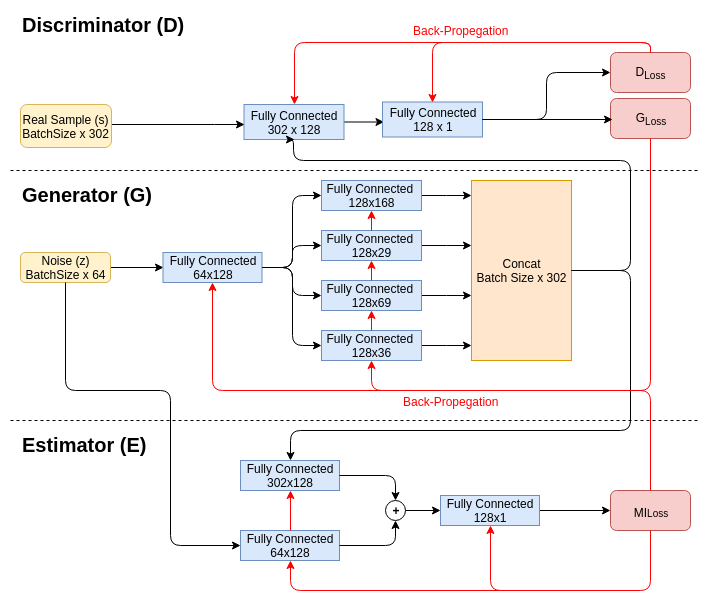
\includegraphics[width=\textwidth]{model_complex}
	\caption{WGAN-GPMI Model}
	\label{fig:model_complex}
\end{figure}

Since mutual information is theoretically unbounded, gradient updates resulting from it could overwhelm the adversarial gradients resulting from the Earthmover Distance. In order to address this all of the gradient updates to the generator are adaptively clipped to ensure that the Frobenius norm of the gradient resulting from the mutual information is at most equal to the adversarial gradient \cite{Belghazi2018}, as shown in (\ref{eq:fnorm}).

\begin{equation}
	g_{norm} = g_a + min(||{g_a}||, ||{g_m}||)({g_m \over ||g_m||})
	\label{eq:fnorm}
\end{equation}
 
Note that $g_{norm}$ is the normalized gradient, $g_a$ is the adversarial gradient resulting from (\ref{eq:WGAN-GP3}), and $g_m$ is the gradient resulting from (\ref{eq:MINE}). 

%\subsection{Model Training}
%\label{sec:training}

%Training GANs is a notoriously tricky task as loss score is not a fair representation of whether the model has converged to generating realistic data. Like many traditional Deep Learning models, hyperparameter tuning is critical to model performance for GANs. This creates a challenge while training GANs, especially with unconventional datasets where metrics like Inception Score cannot be applied. In order to address this and exhaustive hyperparameter search for each of the GAN models above was carried out. First, individual parameters were tuned in order to find candidate values. Then, these candidate values were used in a search of all possible parameter combinations.

%Using the histogram intersection metric proposed in Section \ref{sec:anal} across all combinations of features, the hyperparameter setting which achieved the most intersection scores in the $90^{th}$ percentile were selected as optimal. More details about the result of this search will be covered in Section \ref{sec:rna}.
	\chapter{Analysis Methods}


The usage of NIDS alert data with Machine Learning algorithms suffers from two issues; significant preprocessing must be performed to make the data have contextual meaning and methods to analyze the similarity of alerts are not well defined. For example, predicting a specific port which will be attacked only provides a small piece of significant data. However, a more significant feature to generate would be what type of service will be attacked. Additionally, when analyzing cyber alerts identifying the fidelity of data is not straight forward. In tasks such as event prediction results may be quantified by cross entropy loss on a per feature basis. But when generating new alerts there are complex interactions between various features which must be accounted for by the model. Simply generating \emph{a} realistic signature and port category individually is much less important than generating a realistic \emph{combination} of port signature and category. 

To address these challenges this section will cover the unique preprocessing applied to NIDS data collected from Suricata. Specifically, the features of Alert Signature, Destination Port, Timestamp, and Source IP will be considered. Additionally, intuitive metrics for analyzing alert fidelity are introduced as an inclusive system to address how realisitc generated alerts are compared to their source alerts from the ground truth dataset. Finally, metrics to analyze dependency are introduced and used to verify that high level relationships between alert features are preserved by the model.


\section{Cyber Alert Data Preprocessing}
\label{sec:preproc}

The data used for these experiments comes from the National Collegiate Penetration Testing Competition from 2017 and 2018 (\texttt{https://nationalcptc.org/}). In 2017, teams were tasked with penetrating and exploiting network vulnerabilities in a virtualized network managing election systems. In 2018 teams were required to attack a multifaceted system handling autonomous cars which included host based systems, servers, and mobile assets such as cell phones running an app. Each team had a total of 8 hours to scan, infiltrate the network, and exfiltrate information from the target. Both datasets provide a unique opportunity for Machine Learning experimentation as they are completely comprised of malicious actions as teams attempt to penetrate the target network. Though this data is unique to the competition it is worth noting that the preprocessing described herein is applicable to any dataset consisting of NIDS alerts.  

The first preprocessing step applied to the data was to separate alerts on a per Destination IP basis. This allowed individual models to be trained for each system on the network, typifying the type of traffic seen at that target. Additionally, data from all of the teams could be compounded, allowing for the number of potential attacks taken on a single target to be more fully expressed during training. Segmentation on a per-target basis has several intuitive benefits: First, it allows for different vulnerabilities to be highlighted on each machine given commonly occurring alert features at that target. Secondly, it helps to remove noisy alert influence from critical nodes in the network. For example, internet facing IPs may contain a significant amount of scanning activity, drowning out exfiltration related alert features at nodes further embedded in the network. Finally, the information extracted from alerts on a per target basis is actionable, as network administrators can use commonly targeted vulnerabilities to tune network settings for future defense. 

Next, the dimensionality of the destination port feature was reduced based off common service categories run across a collection of ports provided by the Internet Assigned Numbers Authority \cite{iana}. This reduction drops the number of unique values from 1516 destination ports to 69 destination port categories for the CPTC'17 dataset. Additionally, the dimensionality reduction step can easily be expanded or customized on a per network basis given a corporation's configuration of services. Contextually, this has the effect of indicating what service is being targeted by attackers, rather than just knowing a specific port number. Herein the processed Destination Ports are referred to as Destination Services. 

Finally, a set of simple statistical criterion are used to segment timestamps into bins. Traditional modeling of cyber attacks use killchain stages to segment actions into a series of contiguous stages with dependencies on previous stages. The beginning of an attack may consist of reconnaissance based actions, yielding information about which IP to target in later attack stages. Similarly, the CPTC dataset may be segmented to try and capture unique behaviors into different Time Bins. 

Following the methodology shown by \cite{us} bins are generated by smoothing the histogram timestamps and taking the first derivative to identify local minima and maxima. Then stages are cut if they contain at least $10\%$ of the total data and consecutive events at the candidate point contain less than $0.5\%$ of the total data. The goal of this ruleset is to capture significantly different types of traffic that does not split bursts of data into multiple stages.

Finally, if applied to real world NIDS data, another potential preprocessing step would be to segment source IPs based off of subnet. However, given that CPTC occurs in a virtualized network for a collegiate competition this preprocessing step is ignored. Additionally, it is worth noting that in real world data, the Source IP could easily be obfuscated through the use of a proxy. 


\section{Methods of Analyzing Alert Data}
\label{sec:anal}
Analyzing the degree of realism for artificially generated alert data is non-trivial. While other fields such as Computer Vision have created well defined metrics such as Inception Score \cite{Salimans2016} or allow for direct human analysis of image quality, no analogue exists for NIDS alerts. Several works have proposed the use of graph based metrics such as comparing nodes and their connectivity for both generated and real network traffic \cite{Siska2010, Iannucci}, or looking at low level parameters such as distributions of packets \cite{Sommers2004, Botta2012}. However, despite these works there is no widely accepted methodology.

It is important to consider the desirable attributes of a \emph{good} metric. A good metric must provide an intuitive, scalable way to summarize what would otherwise be an intractable amount of data to comprehend. Other desirable properties include ways to directly visualize the results of the metric so that trends may be identified visually, able to capture high level dependencies, and tolerance to samples with the value $0$. 

To this end, we propose the usage of several metrics for analyzing NIDS alert data. First, histogram intersection is considered; this metric compares the similarity of two histograms within the same domain by computing the amount of overlap between them. Histogram intersection meets several of the above criterion, as it is naturally bounded between 0 and 1, easily visualized by directly plotting the histograms being compared, and can be extended to accommodate m-many tuples of features. The m-many tuples can be thought of as a joint histogram, where $m$ is the number of unique features considered in the joint distribution. This can be done automatically by iterating over all $M$ choose $m$ \emph{combinations}, where $M$ is the total number of unique features in the dataset. Mathematically histogram intersection is defined in (\ref{eq:intersection}), where \emph{gt} represents the ground truth data histogram and \emph{gen} represents the generated data histogram, each of which has $N$ samples.

\begin{equation}
\label{eq:intersection}
G = {{\sum_{i=0}^{N} min(gt_i, gen\_i)} \over {max(\sum_{i=0}^{N} gt_i, \sum_{i=0}^{N} gen_i)}}
\end{equation}

Another powerful trait of histogram intersection is that it can be used to reveal dependencies between features within a single alert. This is accomplished by looking at the difference in histogram intersection scores between $m\pm1$ tuples and observing the intersection drop. An intuitive example of this can be thought of as follows; If the intersection for feature $A$ is 0.9 and the intersection for a 2-tuple histogram consisting of features $A$ and $B$ is $0.875$ then it is expected that a dependency exists between $A$ and $B$. It is important to note that this dependency is not inherently bidirectional, as $A$ and $B$ may have varying intersections to begin with. Fig. \ref{fig:metric_graph} illustrates a graph based schema to identify these dependencies visually. 

\begin{figure}[!htbp]
	\centering%
	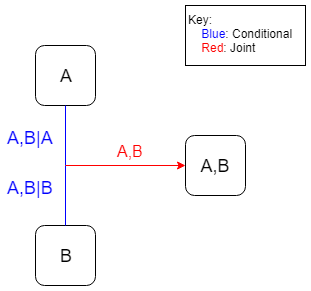
\includegraphics[width=70mm]{metric_graph}
	\caption{
		Example Feature Graph Highlighting Conditional and Joint Entropy
	}
	\label{fig:metric_graph}
\end{figure}

In order to confirm these dependencies we introduce our second metric; conditional entropy. The conditional entropy of each unique \emph{permutation} may be calculated for each m-tuple of features. Continuing with the previous example this means the conditional entropy of both $A|B$ and $B|A$ are computed. In order to compute a single value that represents the average conditional entropy for all input condition values, the entropy term is computed using (\ref{eq:wce}). This calculation weights the entropy of each possible input combination based off the probability that input $i$ occurs as ${{|w_i|} \over {|w|}}$. ${p_{i|j}}$ represents the probability of the output feature value at index $j$ occurring given the input feature values at index $i$ and must be computed for all possible output values $Z$.

\begin{equation}
\label{eq:wce}
\widehat{H}_{Y|X_0, X_1, ..., X_m} = \sum_{i=0}^{N} \bigg({{|w_i|} \over {|w|}} * {\sum_{j=0}^{Z}\Big({p_{i|j} * \log ({1 \over{p_{i|j}}})}\Big)}\bigg)
\end{equation}

In order to further strengthen the argument that there are dependencies between features it is important to consider the overall randomness of the m-tuple joint distribution. To do this (\ref{eq:je}) may be used to compute the joint entropy of the distribution. Using the aforementioned example with features $A$ and $B$, the joint of these variables is denoted $A,B$.

\begin{equation}
\label{eq:je}
{H}_{X_m} = -\sum_{x_m} p(x_0, x_1,...,x_m)  * \log \big({{p(x_0,x_1,...,x_m)}}\big)
\end{equation}

Given that natural logarithms are used for the calculation in (\ref{eq:wce}) and (\ref{eq:je}), the resulting value is given in the natural unit of information (nats), a log base e equivalent to bits. Given that the distribution of m-tuple feature histograms is a discrete distribution with finite support the upper bound of entropy is given by the uniform distribution $mathbb{U}$. Note that the cardinality of $mathbb{U}$ varies to match the number of unique values in the conditional or joint probability being normalized. Using this quantity, (\ref{eq:wce}) and (\ref{eq:je}) can be normalized as shown in (\ref{eq:norm_wce}) and (\ref{eq:norm_je}). This has the benefit of naturally bounding the entropies between 0 and 1, similar to the intersection score defined in (\ref{eq:intersection}).

\begin{equation}
\label{eq:norm_wce}
\overline{H}_{Y|X_0, X_1, ..., X_m} = {{\widehat{H}_{Y|X_0, X_1, ..., X_m}} \over{ H(\mathbb{U})}}
\end{equation}

\begin{equation}
\label{eq:norm_je}
\overline{H}_{X_m} = {{{H}_{X_m}} \over{ H(\mathbb{U})}}
\end{equation}

If the drop in intersections is indeed correlated to feature dependency, then the conditional entropy should be directly proportional to this drop. Additionally, the benefit of capturing feature dependencies is apparent by comparing to the joint entropy without any conditioning information. Note that in Fig. \ref{fig:metric_graph} the edges corresponding to conditional and joint entropies are labeled using the notation given in the examples above.

One drawback of using the intersection of histograms is that the metric does not perform well when the ground truth distribution has one value which occurs with high probability. The data generating model can learn to output that value in a purely deterministic manner and receive an intersection score equivalent to the probability of that given value occurring in the ground truth set. This issue is known as output mode collapse and has been historically problematic for GAN based models. In order to identify this issue a metric which penalizes failure to accurately represent the probability distribution of the ground truth set is required. 

Kullback Leibler Divergence, given in (\ref{eq:kldiv}), was considered as a candidate however it does not have the property of zero tolerance and is asymmetric. This would require special handling of null outputs and would require a defined convention of which probability distribution is considered P and which is given by Q.  

\begin{equation}
	D_{KL}(P||Q) = -\sum_{x \in X}P(x)\log{Q(x) \over P(x)}
\end{equation}

The Jensen Shannon Divergence, given in (\ref{eq:jsdiv}), was then considered. It is both zero tolerant and symmetric while maintaining the penalty for failing to accurately represent the ground truth probability distribution. This metric has the downside of having no upper bound and by extension is not as intuitive as the histogram intersection. However it can be used as a drop in replacement for histogram intersection and can still be used in conjunction with the weighted conditional and joint entropies to identify feature dependency.

\begin{align}
	M(P,Q) &=  {1 \over 2}(P + Q)\label{eq:mid} \\
	D_{JS}(P||Q) &=  {1 \over 2}(D_{KL}(P||M) + D_{KL}(Q||M)) \label{eq:jsdiv}
\end{align}

\section{Other Useful Ways to Analyze Alerts}

The purpose of this section is to review other methods of analyzing artificially generated alerts. The methods presented in this section are comprised of subsidiary steps for the computation of the previously presented metrics and or provide useful information in understanding what is driving model behavior. 

\subsection{Using Conditional Probability Tables to Evaluate Generated Alerts}

In the aforementioned (\ref{eq:wce}) weighted conditional entropy is computed to provide a singular score representing conditional randomness in m-tuple histograms. An intermediary step in this computation involves the creation of conditional probability tables which show all possible input conditioning values and their impact on output value probability. It was found through experimentation that directly outputting these tables and applying highlighting to reveal sparsity and determinism is an effective means to evaluate specific feature value relationships. This method has the drawback of becoming intractable as the number of tables generated is equal to the number of unique feature permutations. A sample table is given in Section \ref{sec:rna} to illustrate specific feature-value relationships.

\subsection{Measuring Output Mode Capture}

One important attribute of artificially generated data is the number of output modes that the model manages to capture. Traditionally, GANs have suffered from output mode collapse, where outputs that have a low probability of occurring in the ground truth do not ever occur in the model's output. This can be thought of as a false negative for the model. Additionally, if the GAN has not been trained sufficiently then there is the potential for it to generate noisy samples which never occurred in the ground truth dataset. This can be thought of as a false positive for the model. 

Generating a table of the false negatives allows for direct testing of the WGAN-GPMI model, which decreases output mode collapse through a mutual information constraint on the generator. Additionally, a table of false negatives allows for direct testing of the amount of noise generated by the model, potentially indicating that more training steps or data is required to obtain realistic results. Ideally, both of these values should be driven towards zero if the model is performing well. Note that this does not indicate a perfect model however, as the probability distribution for output modes may not reflect those of the ground truth distribution. 

	\chapter{Results and Analysis}
\label{sec:rna}

% TODO: Include mention that this spans across 17 and 18 data.

Each of the GAN models described in Section \ref{sec:model_arch} were used to create artificial NIDS alert data.  Using the methods described in Section \ref{sec:meth} the fidelity of the learned model was analyzed. This analysis can be broken down into the following sections:

\begin{enumerate}
	\item Thorough Hyperparameter Search - Individual hyperparameters were tuned for each model to see their impact on histogram intersection. Top candidate values were selected for a full hyperparameter search where all combinations of hyperparameter values. The results are presented for both WGAN-GP and the improved WGAN-GPMI.
	
	\item Alert Fidelity - A subset of target IPs from both the CPTC'17 and CPTC'18 dataset were used for training WGAN-GP and WGAN-GPMI models. The results of these models were analyzed and visualized using histogram intersection and Jensen-Shannon Divergence.
	
	\item Alert Dependency - For the same subset of target IPs alert dependencies were identified by using drop in histogram intersection, entropy computation, and conditional probability tables.
	
	\item Output Modes Captured - The number of output modes captured by the model is comprised of two components. How many of the true output modes are output by the model. And how many output modes by the model do not occur in the ground truth. 

\end{enumerate}

\section{Thorough Hyperparameter Search}
\label{sec:search}
A two part hyperparameter search was employed to find optimal values for generating alerts from the CTPC datasets. First, individual parameters were tested in order to find several values which resulted in promising results. For each parameter value tested, the histogram intersection was computed for all possible feature value combinations. These values were then plotted against all other parameter settings results for WGAN-GP and WGAN-GPMI. Then, these values were taken and used for a full parameter sweep, which tested every possible combination of the parameter values available. Several candidate values were selected for each of the hyperparameters due to the unknown nature of hyperparameter interaction.

This two stage search was carried out twice, once for each of the GAN models presented in Section \ref{sec:model_arch}. The parameters tested included batch size, hidden dimension, learning rate, lambda, and number of epochs.

\subsection{Batch Size}
The batch size determines how many alert samples were fed into the model in parallel. Higher batch sizes can are more computationally intensive, but provide a better representation of the ground truth data distribution. Additionally, larger batch sizes reduce the number of steps required to complete a full epoch of training. 

The values tested for batch size were $\{10, 25, 50, 100, 150, 250, 500, 1000\}$. The intersection vs. parameter setting plots for WGAN-GP and WGAN-GPMI may be seen in Fig. \ref{fig:wgan_batch_size} and Fig. \ref{fig:gpmi_batch_size} respectively.
\begin{figure}[!htbp]
	\centering
	\caption{Batch Size Parameter Search}
	\begin{subfigure}{.7\textwidth}
		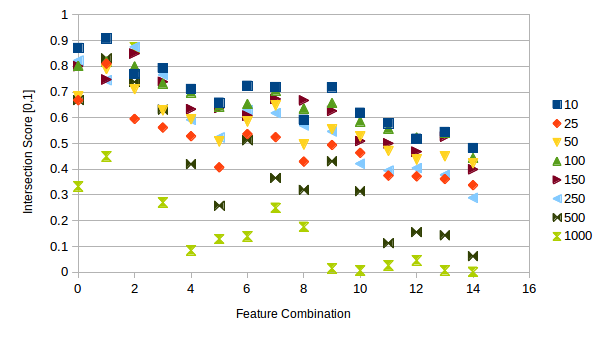
\includegraphics[width=\textwidth]{wgan_batch_size}
	\end{subfigure}%
	\begin{subfigure}{.3\textwidth}
		\caption{
			All other hyperparameters were held constant at the following values: $epochs=180$, $learning\_rate=5e-5$, $hidden\_dimension=128$, $\lambda=0.1$
		}
		\label{fig:wgan_batch_size}
	\end{subfigure}%

	\begin{subfigure}{.7\textwidth}
		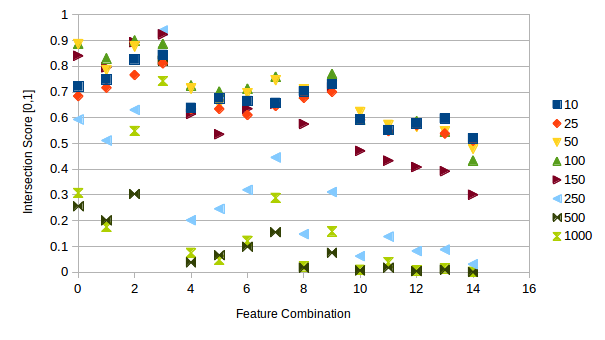
\includegraphics[width=\textwidth]{gpmi_batch_size}
	\end{subfigure}%
	\begin{subfigure}{.3\textwidth}
		\caption{
			All other hyperparameters were held constant at the following values: $epochs=250$, $learning\_rate=5e-4$, $hidden\_dimension=128$, $\lambda=0.3$
		}
		\label{fig:gpmi_batch_size}
	\end{subfigure}%
\end{figure}



% TODO: Analysis

\subsection{Hidden Dimension}
The hidden dimension size determines the number of hidden units available in each hidden layer. Higher hidden dimensions provide more learnable connections to the network allowing the network to complex approximations. On the other hand, larger hidden dimension sizes leads to potential overfitting and raises the computational complexity of training the network. 

The values tested for hidden dimension were $\{64, 128, 256, 384, 512\}$. The intersection vs. parameter setting plots for WGAN-GP and WGAN-GPMI may be seen in Fig. \ref{fig:wgan_hdim} and Fig. \ref{fig:gpmi_hdim} respectively. 

\begin{figure}[!htbp]
	\centering
	\caption{Hidden Dimension Parameter Search}
	\begin{subfigure}{.7\textwidth}
		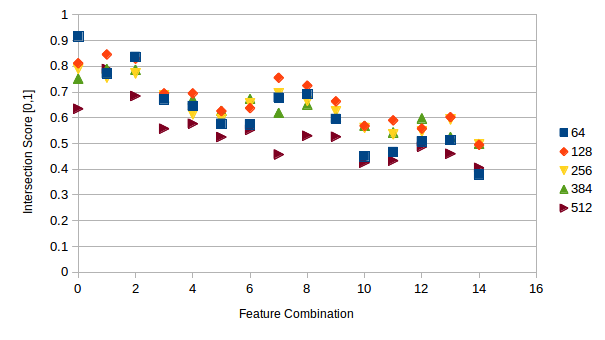
\includegraphics[width=\textwidth]{wgan_hdim}		
	\end{subfigure}%
	\begin{subfigure}{.3\textwidth}
		\caption{
			All other hyperparameters were held constant at the following values: $epochs=180$, $batch\_size = 100$, $learning\_rate=5e-5$, $\lambda=0.1$
		}
		\label{fig:wgan_hdim}
	\end{subfigure}%
	
	\begin{subfigure}{.7\textwidth}
		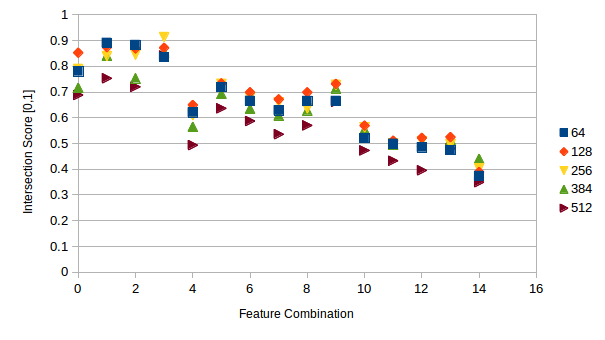
\includegraphics[width=\textwidth]{gpmi_hdim}
	\end{subfigure}%
	\begin{subfigure}{.3\textwidth}
		\caption{
			All other hyperparameters were held constant at the following values: $epochs=250$, $batch\_size=100$, $learning\_rate=5e-4$, $\lambda=0.3$
		}
		\label{fig:gpmi_hdim}
	\end{subfigure}%
\end{figure}


% TODO: Analysis

\subsection{Learning Rate}
The learning rate of the optimizer defines the base step size, weighted by the gradient of the loss, that is taken when adjusting parameter weights during training. A large learning rate converges quickly, but may overshoot the global optimum and never reach peak performance. A small learning rate won't overshoot the global optimum, however will take significantly longer to converge. Due to the categorical output of alert data and existing difficulty in optimizing GANs, small learning rates were tested. This allowed the network to be able to make fine tuned changes to network weights. Additionally, the ADAM optimizer was used, allowing for weight decay over time to modify the learning rate parameter. 


The values tested for learning rate were $\{1e-5, 5e-5, 1e-4, 5e-4, 1e-3\}$. The intersection vs. parameter setting plots for WGAN-GP and WGAN-GPMI may be seen in Fig. \ref{fig:wgan_lr} and Fig. \ref{fig:gpmi_lr} respectively. 

\begin{figure}[!htbp]
	\centering
	\caption{Learning Rate Parameter Search}
	\begin{subfigure}{.7\textwidth}
		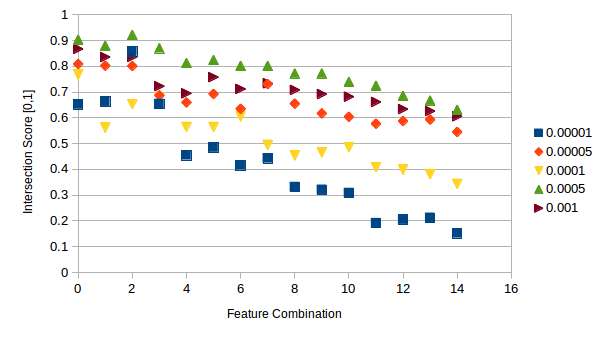
\includegraphics[width=\textwidth]{wgan_lr}
	\end{subfigure}%
	\begin{subfigure}{.3\textwidth}
		\caption{
			All other hyperparameters were held constant at the following values: $epochs=180$, $batch\_size = 100$, $hidden\_dimension=128$, $\lambda=0.1$
		}
		\label{fig:wgan_lr}
	\end{subfigure}%

	\begin{subfigure}{.7\textwidth}
		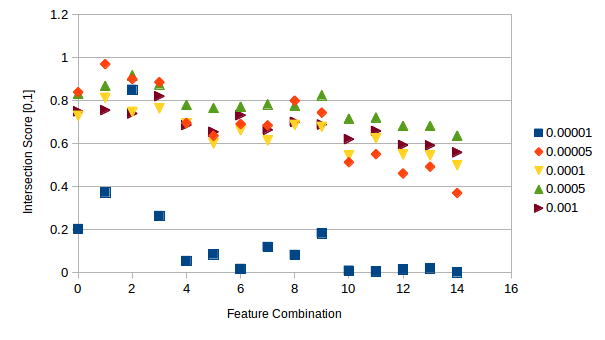
\includegraphics[width=\textwidth]{gpmi_lr}
	\end{subfigure}%
	\begin{subfigure}{.3\textwidth}
		\caption{
			All other hyperparameters were held constant at the following values: $epochs=250$, $batch\_size=100$, $hidden\_dimension=128$, $\lambda=0.3$
		}
		\label{fig:gpmi_lr}
	\end{subfigure}%
\end{figure}


% TODO: Analysis

\subsection{Lambda}
The lambda parameter was used as a coefficient to the gradient penalty term applied to the discriminator. The values tested for lambda were $\{0.05, 0.1, 0.2, 0.3, 0.4\}$. The intersection vs. parameter setting plots for WGAN-GP and WGAN-GPMI may be seen in Fig. \ref{fig:wgan_lam} and Fig. \ref{fig:gpmi_lam} respectively.

\begin{figure}[!htbp]
	\centering
	\caption{Lambda Parameter Search}
	\begin{subfigure}{.7\textwidth}
		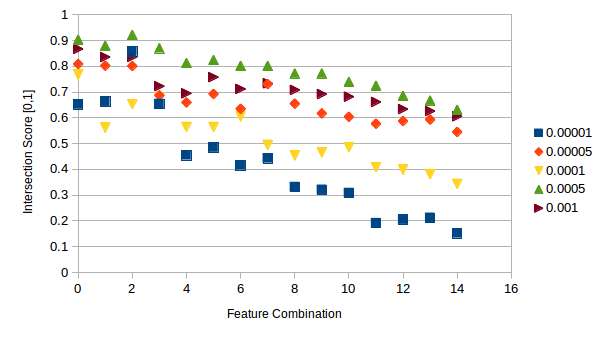
\includegraphics[width=\textwidth]{wgan_lr}
	\end{subfigure}%
	\begin{subfigure}{.3\textwidth}
		\caption{
			All other hyperparameters were held constant at the following values: $epochs=180$, $batch\_size = 100$, $learning\_rate=5e-5$, $hidden\_dimension=128$
		}
		\label{fig:wgan_lam}
	\end{subfigure}%

	\begin{subfigure}{.7\textwidth}
		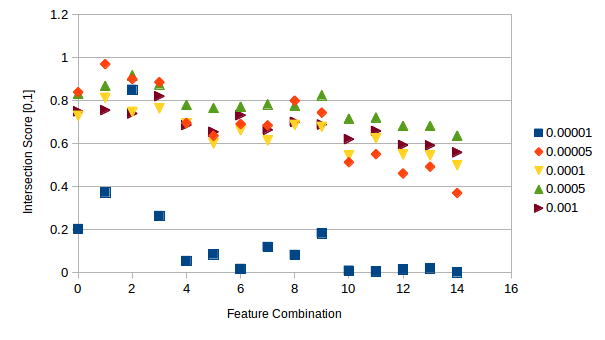
\includegraphics[width=\textwidth]{gpmi_lr}
	\end{subfigure}%
	\begin{subfigure}{.3\textwidth}
		\caption{
			All other hyperparameters were held constant at the following values: $epochs=250$, $batch\_size=100$, $learning\_rate=5e-4$, $hidden\_dimension=128$
		}
		\label{fig:gpmi_lam}
	\end{subfigure}%
\end{figure}


% TODO: Analysis

\subsection{Epochs}
The number of epochs determined how many times the network was exposed to the full dataset during training. Using a large number of epochs allows for the network to get more exposure to the ground truth distribution. However using a very large number of epochs can lead to the network memorizing the data. 

Due to the small size of the CPTC dataset, large values for epochs were tested. These values included $\{50, 100, 150, 200, 250\}$. The intersection vs. parameter setting plots for WGAN-GP and WGAN-GPMI may be seen in Fig. \ref{fig:wgan_epoch} and Fig. \ref{fig:gpmi_epoch} respectively. 

\begin{figure}[!htbp]
	\centering
	\caption{Epochs Parameter Search}
	\begin{subfigure}{.7\textwidth}
		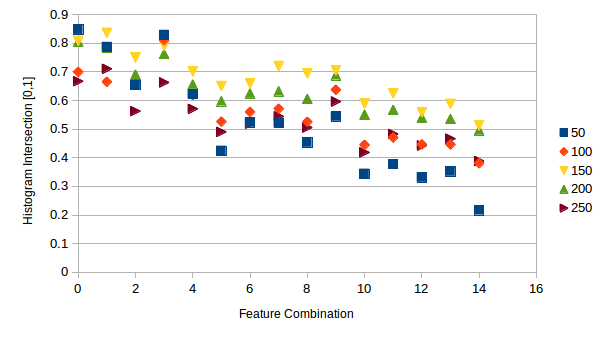
\includegraphics[width=\textwidth]{wgan_epoch}
	\end{subfigure}%
	\begin{subfigure}{.3\textwidth}
		\caption{
			All other hyperparameters were held constant at the following values: $batch\_size = 100$, $learning\_rate=5e-5$, $hidden\_dimension=128$, $\lambda=0.1$
		}
		\label{fig:wgan_epoch}
	\end{subfigure}%

	\begin{subfigure}{.7\textwidth}
		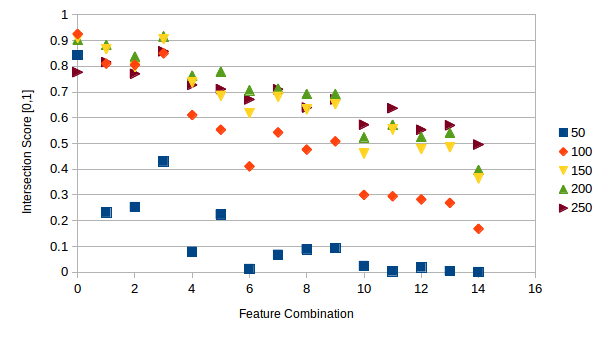
\includegraphics[width=\textwidth]{gpmi_epoch}
	\end{subfigure}%
	\begin{subfigure}{.3\textwidth}
		\caption{
			All other hyperparameters were held constant at the following values: $batch\_size=100$, $learning\_rate=5e-4$, $hidden\_dimension=128$, $\lambda=0.3$
		}
		\label{fig:gpmi_epoch}
	\end{subfigure}%
\end{figure}


% TODO: Analysis


\section{Alert Fidelity}
\label{sec:fidel}



\section{Alert Dependencies}
\label{sec:deped}



\section{Output Modes Captured}
\label{sec:output}



	\chapter{Conclusions and Future Work}

\section{Conclusion}

This work shows the potential for using Generative Adversarial Networks as a means to generate artificial network intrusion detection alerts. Given the stochastic nature of alerts, rarity of known malicious samples, and rapidly growing need for alert data to train Machine Learning algorithms, GANs provide a means to create alerts that traditional statistic models cannot compare to.  

Additionally, two intuitive metrics are defined for analyzing alert generation fidelity; histogram intersection and Jensen Shannon Divergence. Direct visualization of the histogram intersection illustrates the model's output distribution across m-tuple combinations of features, showing the intricacy of learning to output realistic alert data. Jensen Shannon Divergence is employed to confirm relationships identified by histogram intersection and highlight crucial differences in the probability distribution of the generative model.

Using these metrics and information theoretic calculations, feature dependencies are revealed and examined to provide a deeper understanding of both the power and shortcomings of GANs applied to NIDS alert generation. Joint entropy is computed for the ground truth distribution and used as a baseline score identifying the challenge of modeling the data distribution. Then conditional entropy is employed on both the ground truth and generated data distributions to identify feature dependencies and how well the generative network models these dependencies. In order to view low level feature-value dependencies, conditional probability tables are generated and highlighted to show sparsity and determinism. 

Finally, it is shown that using mutual information is an effective means of regularizing the generator network, improving exploration of the ground truth feature space. Not only do the metrics measuring alert fidelity improve, but output mode collapse is shown to decrease. This is a direct result of the generator more closely modeling the ground truth data distribution. 

\section{Future Work}

Though this work shows the promise of GANs in NIDS alert generation the results are far from perfect. Modeling the distribution of alerts is still a monumental challenge for several reasons: The lack of known malicious alert data makes it challenging to train GANs. Current Machine Learning methods in the field of Cyber Security use sequences of alerts in order to model temporal relationships in an attack sequences. And the quality of results requires improvement before being ready for application to other Cyber Security Machine Learning systems.

\subsection{Multi-Alert Generation and Analysis}

Altering the models presented by this work to generating multiple temporally related alerts at once would greatly increase the utility of generator outputs. Current works applying Machine Learning methods to Cyber Security problems almost exclusively use Recurrent Neural Network structures for attack classification and prediction. It is well established that cyber attacks have intricate behavioral patterns consisting of multiple actions; several alerts may be all related to a single goal or exploit used by the attacker. Modifying the models presented to output chains of alerts would allow for inspection of attacker behaviors and long term strategies. 

Two means of modifying these models are presented. First, each of the neural networks presented could be modified to use a Recurrent Neural Network structure. Particularly, Long Short Term Memory cells have been effective at learning complex temporal relationships and can adaptively select when to forget prior information. In order to train a model consisting of LSTM Neural Networks, the ground truth data would have to be segmented into contiguous chains of alerts. Additionally, alert chain generation would have be cut manually, as there is no natural concept of what type of alert marks the end of a chain (whereas in other tasks like sentence generation a period represents the end). 

The second modification to network structure would be to implement Convolutional Neural Networks for each model. In order to make this network structure work, packets would have to be structured into 2D arrays consisting of contiguous alerts. One example of this would be for each packet to have the prior 2 packets preprended to the alert and the subsequent 2 packets appended. This would create an $2N+1$ x $M$ array where $2N+1$ is the number of alerts considered in each input to the network and M is the number of features given by each alert. This network would also have the drawback of being a fixed size input and output. 

Regardless of the means used to generate chains of alerts, new analysis options are immediately available when considering alert sequences. Sequences of alerts could be modeled as Markov Chains allowing for longest common subsequence to be identified and direct comparison of state transition probabilities. This allows for a rich understanding of the temporal performance of the GAN and how it's results differ from ground truth sequences. Additionally alert sequences could be viewed as a graph allowing for visualization of alerts with low connectivity/deterministic attack behavior, and feature value changes over time. 


\subsection{Improving Generation through Reinforcement Learning}

Methods of establishing generator loss in a generative adversarial networks fail to capture discrete features which have interdependencies. This work proposes a way to model generator loss as a game and apply a reinforcement learning inspired solution to it. 

Consider the generator to be an agent, whose action space is comprised of all the potential output features it may generate. Then, consider the following  hierarchical reward scheme: For each feature that is output correctly reward the generator with $2^1$ 'points'. For each pair of features reward the generator with $2^2$ 'points'. And so on and so forth where the maximal reward is $2^n$ 'points'. The n-many tuple that is correct can be considered the order of the output (e.g.) The above examples would be first order, second order, and finally n-th order. This can be established as a sum of the correct combinations as follows: Given A is the action space consisting of all unique features in the dataset	and s is a sample action generated by the neural network drawn from A.

\begin{equation}
L = \sum_{k=1}^{n}\sum_{s_{{(^n_k)}} \in A_{(^n_k)}} 2^k
\end{equation}

This formulation has the following benefits:
\begin{enumerate}
	\item Encourages a generator which captures inter-feature dependencies during training
	\item Can be trained without the discriminator network, lowering the potential intractability of complex networks
	\begin{itemize}
		\item Note that this comes at the expense of a loss funciton with O(n!) runtime, arguably intractible for actions with a high rank
	\end{itemize}
	\item Can be modified to target only a specific combination of features
	\item Increases reward size non-linearly to as to acccount for the significant difficulty increase in getting n-many tuples correct.
\end{enumerate}

Another benefit of formulating loss in this manner is that it allows for easy expandability. Two examples are as follows: 
\begin{enumerate}
	\item The loss may be modified to provide a reward proportional to the probability of the selected character being generated. 
	\item The loss may be modeled as a n-th order Markov Source to capture temporal structure within the data. 
\end{enumerate}

The probability mass function for cyberattack data does not follow any conventional distribution (Normal, Poisson, Uniform, etc), nor does it account for all possible features in the 'Alert Space' [Explain this]. In order to account for this in the loss function each feature predicted that is in the Alert Space would have a weighted reward value by the probability of that feature value occurring as shown below: Let F be a subset of features from the Alert Space A and $F_v$ represents a specific value for the Feature f
\begin{gather}
p_{v_n} = {|F_{v_n}| \over |F_n|}\\
L = \sum_{k=1}^{n}\sum_{s_{{(^n_k)}} \in A_{(^n_k)}} (2^k)p(v_1)
\end{gather}


This can be further expanded to account for the inpact of other features on the target prediction feature. Conceptually, if trying to compute the loss of feature A given feature B as a prior, the conditional probability of A may be computed. This would further encourage inter-feature dependency. 

An example of this would be computing the probability of a specific value for Destination Port given that the value for IP is already determined to be 129.21.154.3. On the other hand, it is still important to value results which occur in the global action space even if they don't occur with the specific IP value given; the intuition behind this is that the generated should also be encouraged to explore the action space, not just exploit it. To do this the joint probability should be used with the naive probability proposed above. 

\begin{gather}
L = \sum_{k=1}^{n-1}\sum_{s_{{(^n_k)}} \in A_{(^n_k)}} (2^k)p(v_1) + \sum_{k=1}^{n-1}\sum_{s_{{(^n_k)}} \in A_{(^n_k)}} (2^k)p(v_1|v_2)
\end{gather}

Such a conditional probability model can also be used to model temporal relations within the data. This is accomplished by using the previous alerts feature value as a prior for the current generated feature. This in turn can be extended to an n-th order markov model where n alert features act as priors for the current feature being generated. This may be represented as shown below:

\begin{gather}
L =  \sum_{k=1}^{n-1}\sum_{s_{{(^n_k)}} \in A_{(^n_k)}} (2^k)p(v_1|v_2, v_3, ..., v_n))
\end{gather}


	
	% Post chapter stuff
	% epilogue.tex
%
% Author       : James Mnatzaganian
% Contact      : http://techtorials.me
% Date Created : 08/27/15
%
% Description  : The epilogue used by "thesis.tex".
%
% Copyright (c) 2015 James Mnatzaganian

% NOTE: All filler text has "TODO" written. This must be removed in the final copy!

% Bibliography
\bibliography{thesis}
\bibliographystyle{plain}

% Glossary
\printglossary[type=main]

\begin{appendices}
	
	\chapter{SVM Feature Dependency Experiment}
	\label{sec:svm_app}
	
	
	One additional way to confirm the dependencies highlighted through drop in histogram intersection and conditional entropy is to test with a simple model for separation. To do so, a SVM with the RBF Kernel function was trained using all unique permutations of features. The model was given 1 to $n-1$ features as conditioners and an expected output feature for all possible input-output pairs. 
	
	To further prove that the dependencies identified by the GAN exist, a SVM was fit to the same $1|2$-combination histograms discussed in Fig. BLANK. The accuracy of this fit was tabulated for all four victim IP addresses tested in Table \ref{table:svm_accuracy}.
	
	\begin{table}[!htbp]
		\caption{SVM Prediction Accuracy For 3-Combination Feature Values Assorted Victim IPs}
		\label{table:svm_accuracy}
		\centering
		\begin{tabular}{l|cccc}
			\multicolumn{1}{l|}{} & \multicolumn{4}{c|}{\textbf{Machine IP Address}} \\
			\multicolumn{1}{l|}{\textbf{Prediction{\given}Features}} & \multicolumn{1}{l}{\textbf{10.0.0.100}} & \multicolumn{1}{l}{\textbf{10.0.0.27}} & \multicolumn{1}{l}{\textbf{10.0.0.22}} & \multicolumn{1}{l|}{\textbf{10.0.99.143}} \\ \hline
			\multicolumn{1}{l|}{\textbf{D{\given}A,T}} & \multicolumn{1}{c|}{0.958} & \multicolumn{1}{c|}{0.591} & \multicolumn{1}{c|}{0.949} & \multicolumn{1}{c|}{0.908} \\
			\multicolumn{1}{l|}{\textbf{D{\given}A,S}} & \multicolumn{1}{c|}{0.962} & \multicolumn{1}{c|}{0.616} & \multicolumn{1}{c|}{0.970} & \multicolumn{1}{c|}{0.977} \\
			\multicolumn{1}{l|}{\textbf{D{\given}S,T}} & \multicolumn{1}{c|}{0.790} & \multicolumn{1}{c|}{0.541} & \multicolumn{1}{c|}{0.879} & \multicolumn{1}{c|}{0.794} \\
			\multicolumn{1}{l|}{\textbf{A{\given}D,T}} & \multicolumn{1}{c|}{0.911} & \multicolumn{1}{c|}{0.490} & \multicolumn{1}{c|}{0.929} & \multicolumn{1}{c|}{0.472} \\
			\multicolumn{1}{l|}{\textbf{A{\given}S,D}} & \multicolumn{1}{c|}{0.852} & \multicolumn{1}{c|}{0.516} & \multicolumn{1}{c|}{0.889} & \multicolumn{1}{c|}{0.486} \\
			\multicolumn{1}{l|}{\textbf{A{\given}S,T}} & \multicolumn{1}{c|}{0.749} & \multicolumn{1}{c|}{0.440} & \multicolumn{1}{c|}{0.811} & \multicolumn{1}{c|}{0.344} \\
			\multicolumn{1}{l|}{\textbf{S{\given}A,T}} & \multicolumn{1}{c|}{0.719} & \multicolumn{1}{c|}{0.742} & \multicolumn{1}{c|}{0.539} & \multicolumn{1}{c|}{0.702} \\
			\multicolumn{1}{l|}{\textbf{S{\given}D,T}} & \multicolumn{1}{c|}{0.736} & \multicolumn{1}{c|}{0.814} & \multicolumn{1}{c|}{0.525} & \multicolumn{1}{c|}{0.729} \\
			\multicolumn{1}{l|}{\textbf{S{\given}A,D}} & \multicolumn{1}{c|}{0.962} & \multicolumn{1}{c|}{0.616} & \multicolumn{1}{c|}{0.970} & \multicolumn{1}{c|}{0.977} \\
			\multicolumn{1}{l|}{\textbf{T{\given}A,S}} & \multicolumn{1}{c|}{0.411} & \multicolumn{1}{c|}{0.387} & \multicolumn{1}{c|}{0.215} & \multicolumn{1}{c|}{0.459} \\
			\multicolumn{1}{l|}{\textbf{T{\given}S,D}} & \multicolumn{1}{c|}{0.408} & \multicolumn{1}{c|}{0.424} & \multicolumn{1}{c|}{0.161} & \multicolumn{1}{c|}{0.514} \\
			\multicolumn{1}{l|}{\textbf{T{\given}A,D}} & \multicolumn{1}{c|}{0.178} & \multicolumn{1}{c|}{0.208} & \multicolumn{1}{c|}{0.189} & \multicolumn{1}{c|}{0.436} \\
		\end{tabular}
	\end{table}
	
	Note that the order of the combinations is the same as that given in Fig. \ref{fig:weighted_conditional_entropy} and held constant for all victim IPs. Though some general trends exist, such as alert signature and destination port category being poor predictors of timestamp, there is variation between the different victims. Fig. \ref{fig:entropy_v_accuracy} shows that regardless of what feature dependencies exist for a given victim there is a strong negative correlation between accuracy of an SVM predictor and the conditional entropy.
	
	\begin{figure}[!htbp]
		\centering
		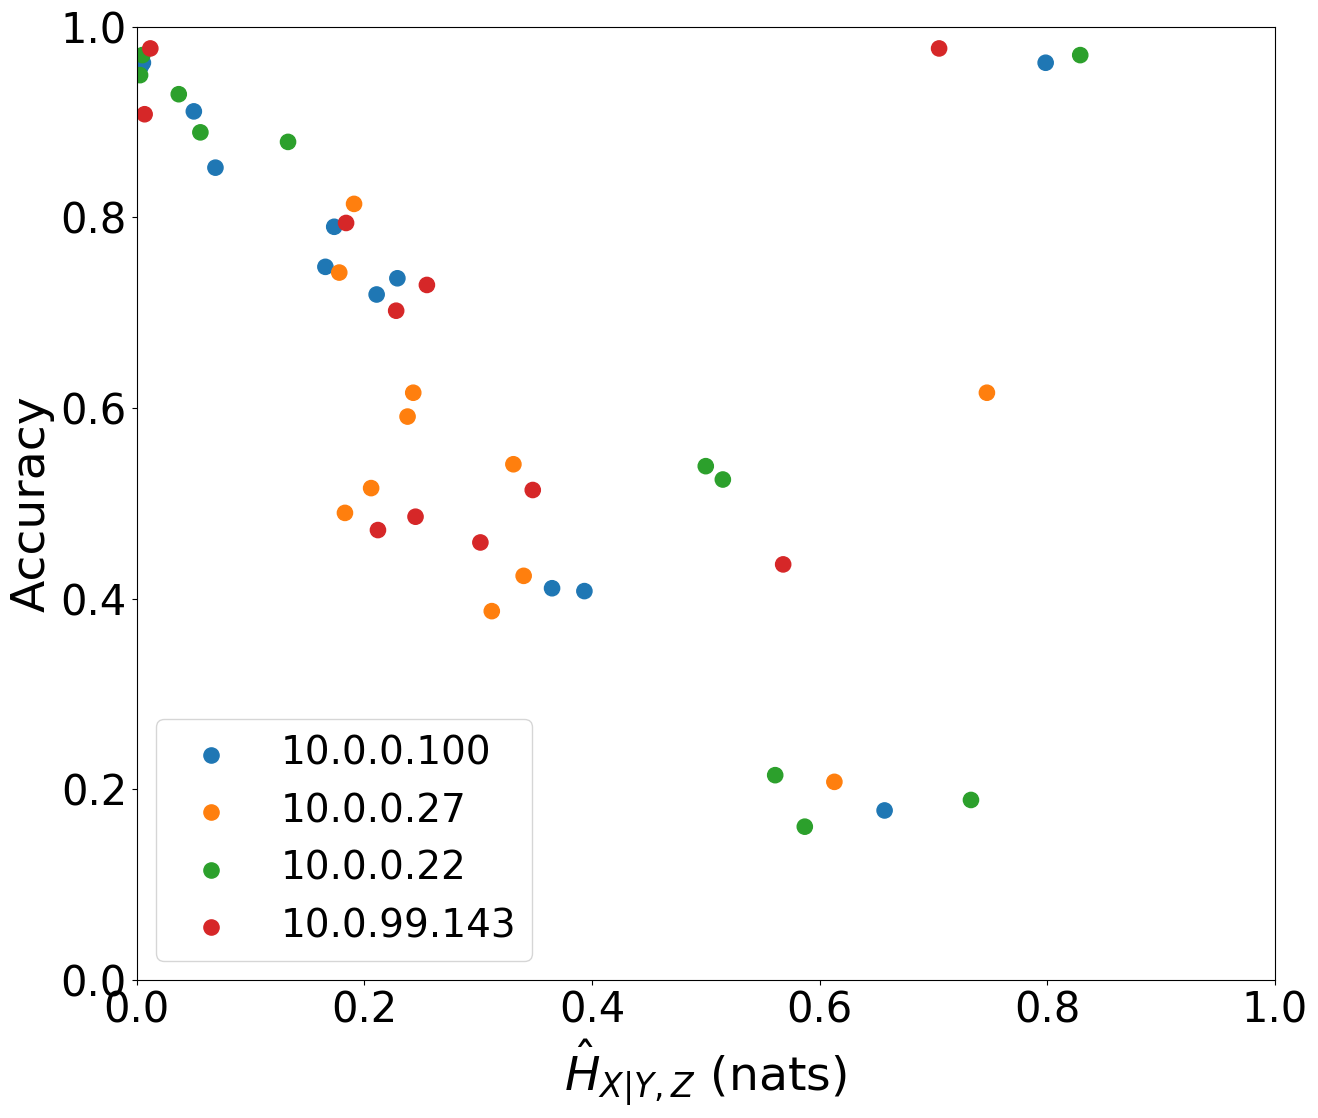
\includegraphics[width=.75\textwidth]{entropy_vs_accuracy.png}
		\caption{SVM Accuracy Plotted Against Conditional Entropy}
		\label{fig:entropy_v_accuracy}
	\end{figure}
	
	
	\chapter{Alert Dependency Plots}
	\label{sec:depend_app}
	
	\begin{figure}[!htbp]
		\centering
		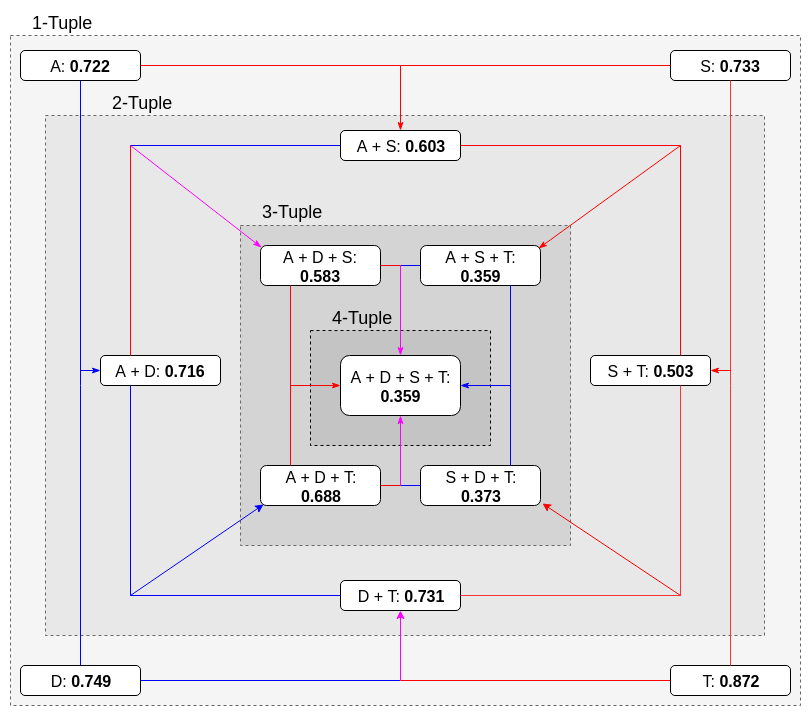
\includegraphics[width=.8\textwidth]{planar_combinations_v3}
		\caption{
			Target 10.0.0.22 Alert Dependency Graph
		}
		\label{fig:alert_depend_2}
	\end{figure}
	
	\begin{figure}[!htbp]
		\centering
		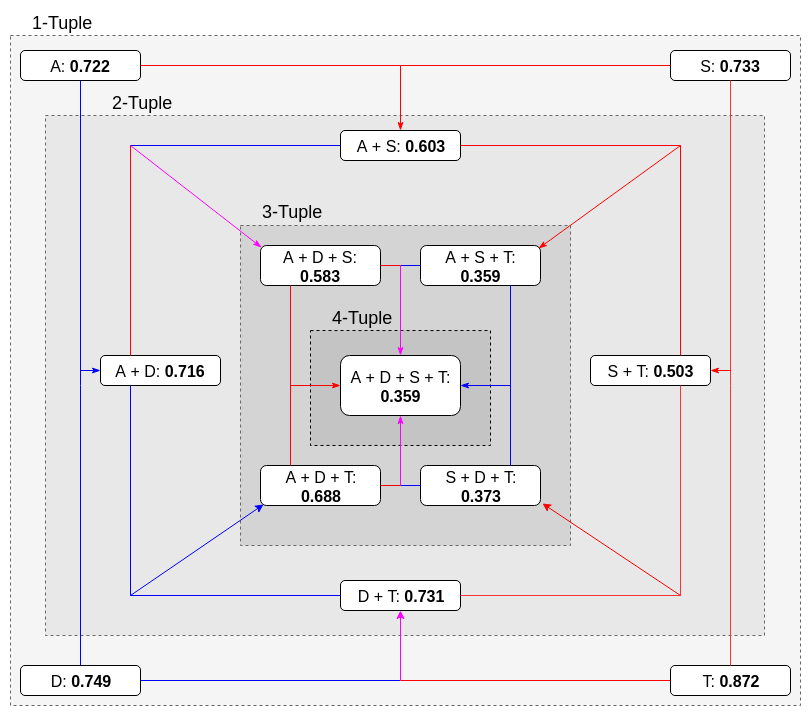
\includegraphics[width=.8\textwidth]{planar_combinations_v3}
		\caption{
			Target 10.0.0.27 Alert Dependency Graph
		}
		\label{fig:alert_depend_3}
	\end{figure}
	
	\begin{figure}[!htbp]
		\centering
		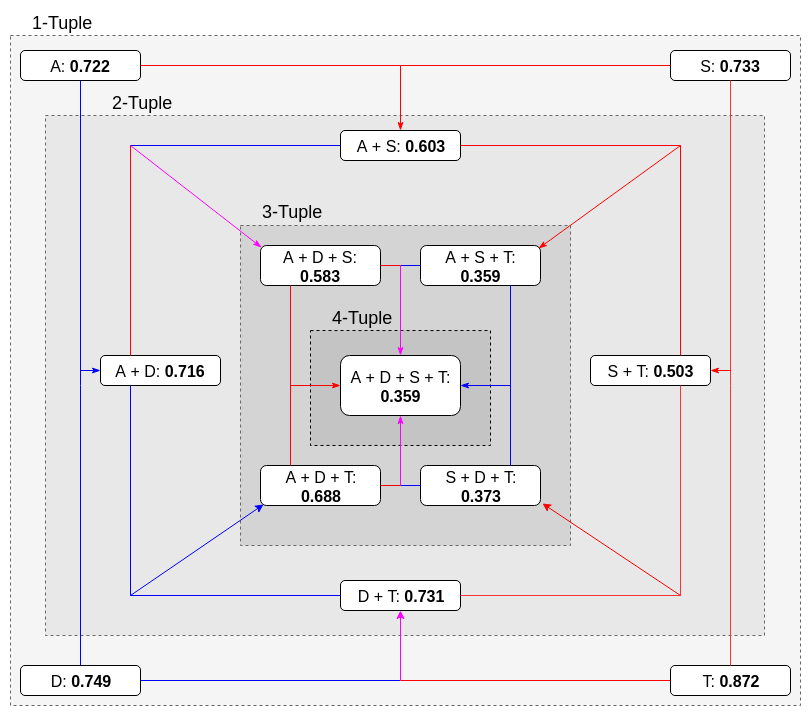
\includegraphics[width=.8\textwidth]{planar_combinations_v3}
		\caption{
			Target 10.0.99.143 Alert Dependency Graph 
		}
		\label{fig:alert_depend_4}
	\end{figure}

	\begin{figure}[!htbp]
		\centering
		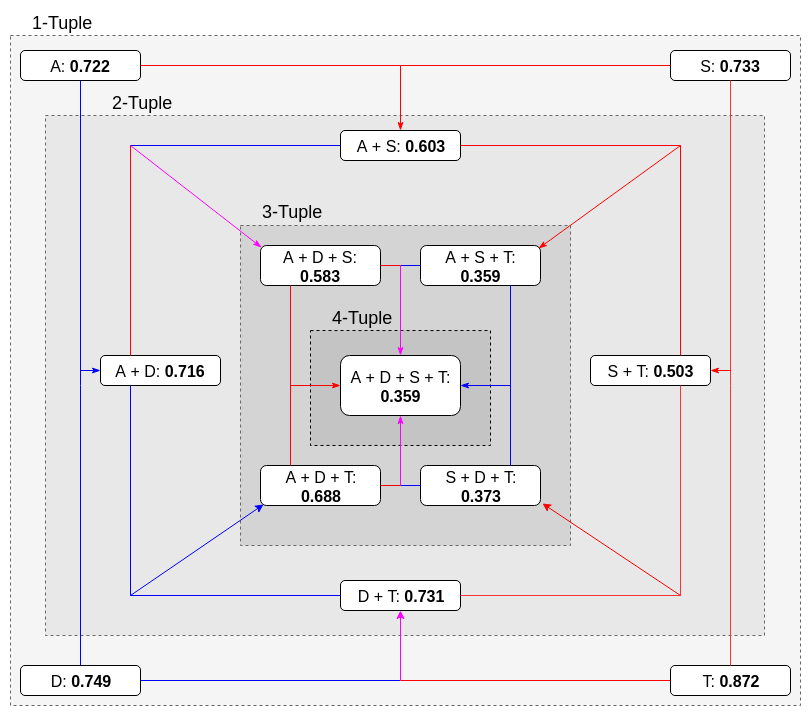
\includegraphics[width=.8\textwidth]{planar_combinations_v3}
		\caption{
			Target 10.0.0.22 Alert Dependency Graph
		}
		\label{fig:alert_depend_6}
	\end{figure}
	
	\begin{figure}[!htbp]
		\centering
		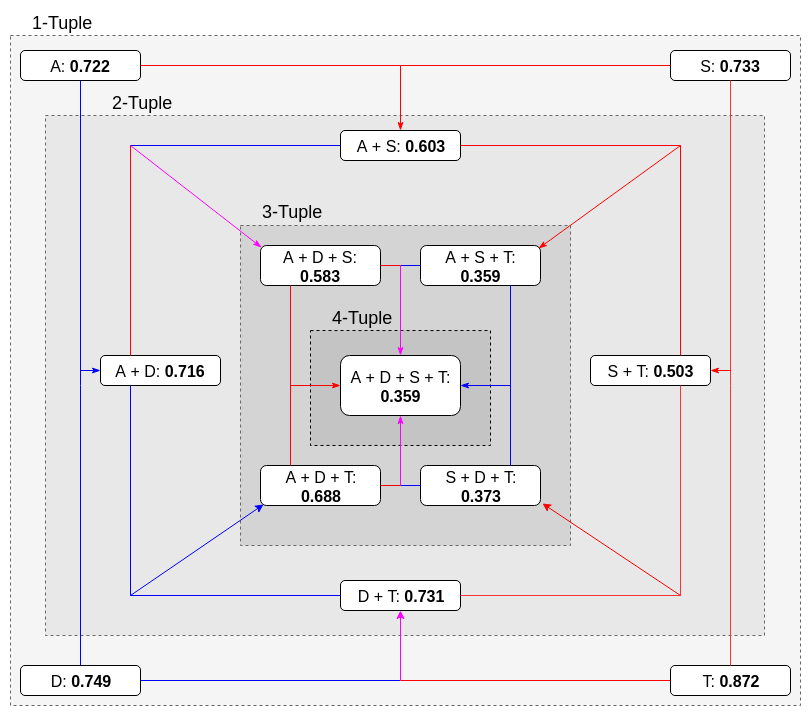
\includegraphics[width=.8\textwidth]{planar_combinations_v3}
		\caption{
			Target 10.0.0.27 Alert Dependency Graph
		}
		\label{fig:alert_depend_7}
	\end{figure}
	
	\begin{figure}[!htbp]
		\centering
		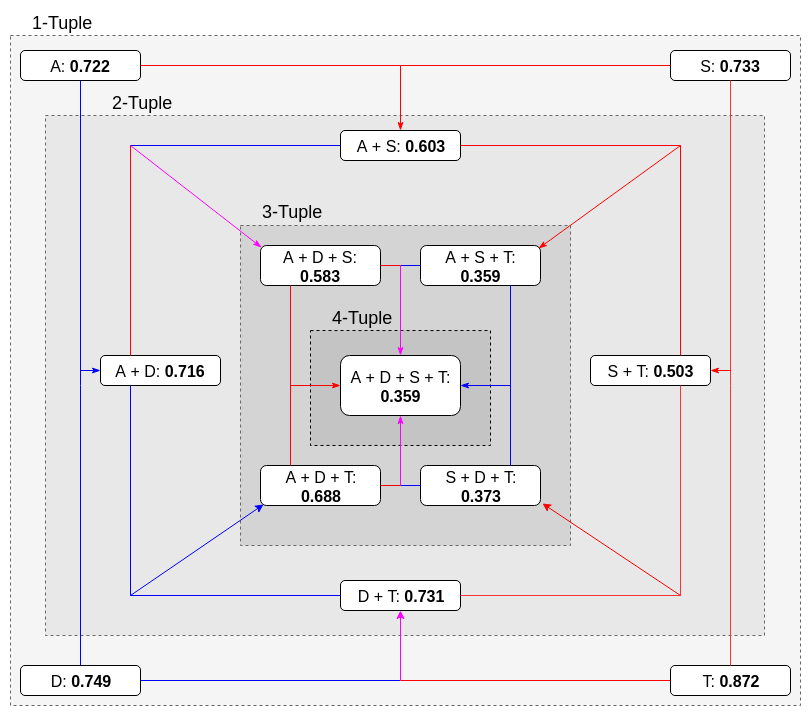
\includegraphics[width=.8\textwidth]{planar_combinations_v3}
		\caption{
			Target 10.0.99.143 Alert Dependency Graph 
		}
		\label{fig:alert_depend_8}
	\end{figure}

\end{appendices}

% End the document
\end{document}